\documentclass[]{style/ceurart}
\sloppy

\usepackage{listings}
\lstset{breaklines=true}

\begin{document}

\copyrightyear{2024}
\copyrightclause{Copyright for this paper by its authors.
  Use permitted under Creative Commons License Attribution 4.0
  International (CC BY 4.0).}

\conference{CLEF 2024: Conference and Labs of the Evaluation Forum, September 9-12, 2023, Grenoble, France}

\title{Tiled Raster Compression and Embeddings for Multilabel Classification in GeoLifeCLEF 2024}

\author[1]{Anthony Miyaguchi}[
orcid=0000-0002-9165-8718,
email=acmiyaguchi@gatech.edu,
]
\cormark[1]
\author[1]{Patcharapong Aphiwetsa}[
email=paphiwetsa3@gatech.edu,
]
\author[1]{Mark McDuffie}[
email=mmcduffie8@gatech.edu,
]

\address[1]{Georgia Institute of Technology, North Ave NW, Atlanta, GA 30332}
\cortext[1]{Corresponding author.}

\begin{abstract}
    This is the abstract of the paper. 
    It should be a brief summary of the contents of the paper.
\end{abstract}

\begin{keywords}
  LaTeX class \sep
  paper template \sep
  paper formatting \sep
  CEUR-WS
\end{keywords}


\maketitle

\section{Introduction}

GeoLifeCLEF is a task organized within the LifeCLEF lab in the CLEF 2024 conference. 
The goal of GeoLifeCLEF is to predict what plant species are present and absent at a specific location given spatial and temporal remote sensing data. 
Being able to model species density distributions can be useful for biodiversity management and conservation among other things.

In this project, we explore methods to solve the posed multilabel classification task and try to incorporate unsupervised methods for building useful representations from the data. 
A large portion of the work spent this semester was focused on preprocessing the data from the competition for modeling, as well as experimenting with various modeling approaches to deal with computational challenges related to the large label space.

\section{Data and Evaluation}

The competition has three major components. 
The first are the metadata associated with the competition comprising a presence-only training, presence-absence training, and presence-absence test set. 
The metadata provides a mapping between location and the species labels available for supervised training. 
The second are the remote-sensing and raster data provided in pixel format. 
The final component is time series data containing quarterly environmental data over a 20 year period. 

The presence-only training dataset comprises 5M examples over 4M survey sites that are distributed across western Europe. 
The presence-absent dataset data of a similar schema, but the semantics are stricter – species that are not included in the survey are known to be not present. 
This is not necessarily the case with the present-only data since they are scraped from crowd-sourced data, meaning that there may be gaps in which species are reported. 
The datasets include an identifier for the survey site and the latitude and longitude. 
We compute a projection into EPSG 3035, which allows for euclidean distance in units of meters. 

\begin{lstlisting}[caption={Number of survey identifiers per dataset.}, captionpos=b,label={lst:counts}]
  +--------+-------+
  | dataset|  count|
  +--------+-------+
  |  	 po|5079797|
  |pa_train|1483637|
  | pa_test|   4716|
  +--------+-------+  
\end{lstlisting}

\begin{lstlisting}[caption={Schema of the metadata.}, captionpos=b,label={lst:schema}]
  |-- dataset: string (nullable = true)
  |-- surveyId: integer (nullable = true)
  |-- lat_proj: double (nullable = true)
  |-- lon_proj: double (nullable = true)
  |-- lat: double (nullable = true)
  |-- lon: double (nullable = true)
  |-- year: integer (nullable = true)
  |-- geoUncertaintyInM: double (nullable = true)
  |-- speciesId: double (nullable = true) 
\end{lstlisting}

The raster and satellite imagery accounts for the majority of the available data. 
We are provided GeoTIFF files for various measures such as elevation, roads, population, and soil. 
The GeoTIFF files are bounded by a GeoJSON polygon that covers western Europe. 
The provided RGB-NIR satellite imagery is provided directly as tiles associated with each survey site.

\begin{lstlisting}[caption={GeoJSON polygon for region specified by GeoLifeCLEF 2024.}, captionpos=b,label={lst:polygon}]
  {
    "type": "Polygon",
    "coordinates": [
        [
            [-32.26344, 26.63842],
            [-32.26344, 72.18392],
            [35.58677, 72.18392],
            [35.58677, 26.63842],
            [-32.26344, 26.63842],
        ]
    ],
}
\end{lstlisting}

\subsection{Processing Raster Data}

The GeoTIFF files need to be processed to use within a supervised learning process. 
There can be significant in-memory overhead with tiling the data, since we need to store the 128x128 byte array for each survey site. 
We fork the official plantnet/GeoLifeCLEF data loaders to pre-compute tiles for each of the provided GeoTIFF under 1GB. 
Certain rasters do not fit into memory (e.g. elevation raster at 11GB), and therefore we omit them from our experiments. 
We only compute the tiles that are associated with the survey identifiers in our metadata which helps with limiting the size of the resulting dataset. 
In addition to generating tiled images, we compute the 2D-DCT on the resulting tile images and keep low-frequency coefficients for as features in downstream modeling. 

\begin{figure}
    \centering
    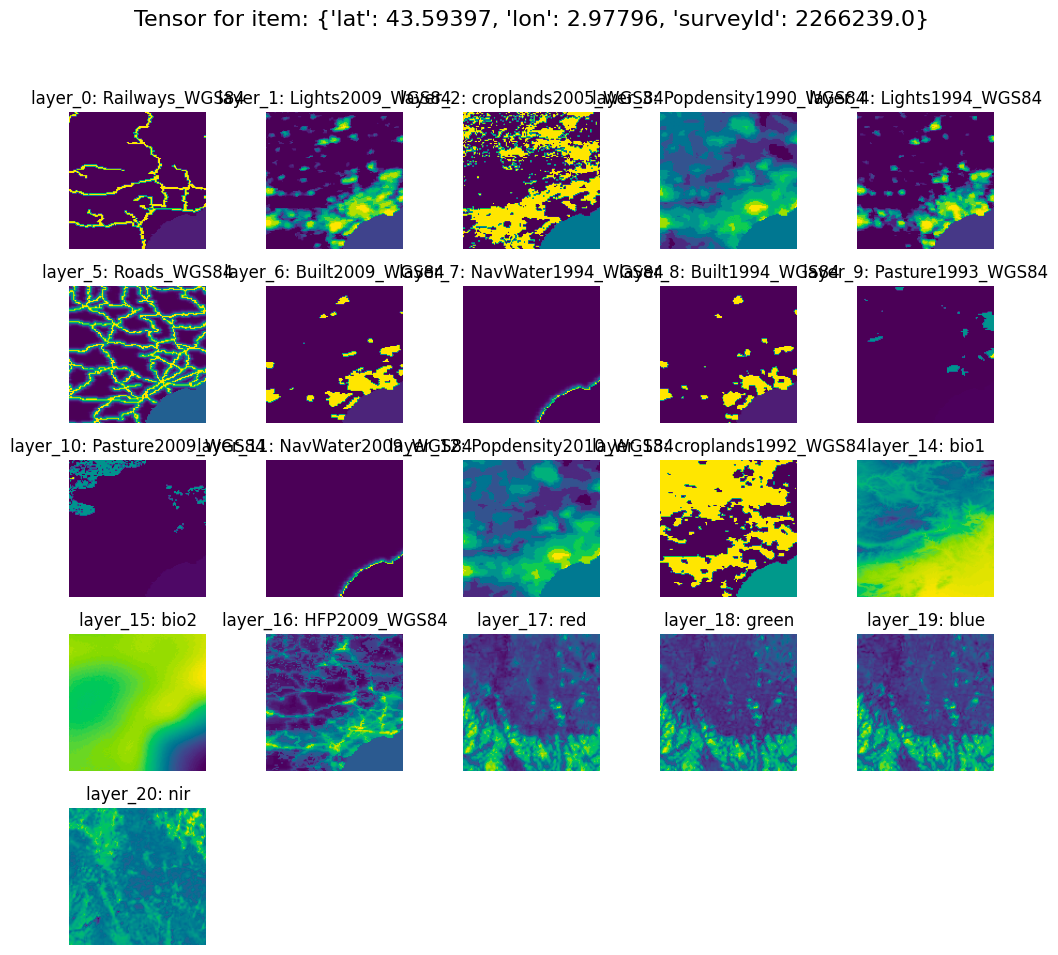
\includegraphics[width=0.9\textwidth]{figures/tiled-raster.png}
    \caption{
        Example of a tiled raster image. 
        The image is a 128x128 tile of the RGB-NIR satellite imagery. 
        The image is associated with a survey site and is used as input to the model. 
    }
    \label{fig:tiled-raster}
\end{figure}

We implement a wrapper around the ND-DCT that we can use in Spark. 
While we do have access to a 1D-DCT for feature preprocessing, we lose a significant amount of information if we simply flatten the image and take the coefficients from that transform.

% three images side by side
\begin{figure}
  \centering
  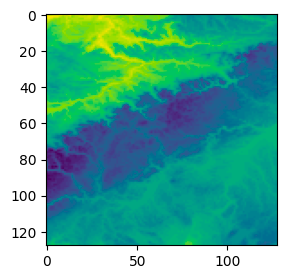
\includegraphics[width=0.3\textwidth]{figures/dct-original.png}
  \hfill
  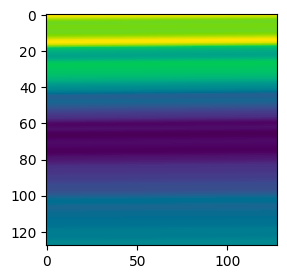
\includegraphics[width=0.3\textwidth]{figures/dct-1d-lowpass.png}
  \hfill
  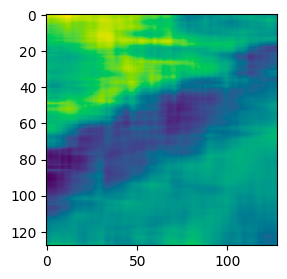
\includegraphics[width=0.3\textwidth]{figures/dct-2d-lowpass.png}
  \caption{
    Example of low-pass filtering using the DCT.
    (a) Original bio1 raster image.
    (b) Low-pass filter using the first 50 coefficients of the 1D-DCT, reshaping on the first axis (row-major order).
    (c) Low-pass filter using the 2D-DCT using the top-left 8x8 coefficients.
  }
  \label{fig:dct-lowpass}
\end{figure}

\section{Experiments}

We run the gamut in trying to build a solution multi-label classification problem. 
Our general approach to solve the species distribution estimation from the given remote-sensing data is to formulate a version of the problem that can be easily expressed in our tooling of choice. 
We use Luigi as our workflow management tool, which is easy to set up and provides idempotent directed acyclic graphs (DAGs) of tasks. 
We use Spark for performing data extraction, transforming, and loading (ETL) from tarred images and csv files to columnar parquet files. 

\subsection{Naive Multi-class Classification}

Our first goal is to learn a relationship between geospatial features (latitude and longitude) and the species labels. 
Our first model is to learn a linear relationship between the features and response using a logistic regression to put together a simple baseline. 
This model is analytically simple, and can be learned using Spark via stochastic gradient descent (SGD). 
As a validation, we build a model using the top-10 species by frequency and find that we obtain an accuracy of 0.09, which is better than random but roughly equivalent to always choosing the most frequent species.

When we decide to scale up the process to using all 5 million rows and 10,358 species, we immediately run into computational issues. 
When we try to fit a logistic regression using scikit-learn or statsmodels, we quickly run into out-of-memory (OOM) issues. 
When we run the same procedure in Spark, we are able to configure a model that takes advantage of the distributed dataframe paradigm. 
However, we find that SGD will run for over 48 hours on a GCP n1-standard-8 instance (8 vCPU, 16GB RAM, 350GB NVME SSD) using 3-fold cross-validation (CV). 
We suspect that this is due to the size of the coefficients that need to be carried around, which involves J features and K output classes. 
Presuming an 8-byte double, the coefficients alone will be at least 8mb which is larger than the typical CPU cache. 
We also note that SGD is an iterative algorithm, and may take a significant amount of time to converge.

We investigate other algorithms for modeling classification, including Naive Bayes, SVM, Random Forests, and Factorization Machines.
Naive Bayes assumes non-negative count data. 
SVMs are not tractable for our problem, and have been found to be slower than linear/logistic regression for other problems in the Spark toolbox. 
Random Forests only support up to 100 classes in Spark, likely due to the branching factor required for making a decision for each class. 
Factorization machines suffer a similar issue to Logistic Regression and SVMs, since this too is computed via SGD. 
Our final attempt to model multi-class classification via classical supervised techniques is through XGBoost, which maintains a Spark binding. 
We find that we quickly run out of memory when trying to model the large number of classes. 

We are unable to model a relationship between latitude and longitude to the species labels with classical machine learning techniques. 
Due to the computational issues that we ran into, we decided to try out other techniques that are tractable with the resources available. 

\subsection{Low-rank Multilabel-Space Regression}

Instead of trying to learn the mapping between features and label-space directly, we attempt several techniques to learn a relationship between features and a low-rank multi-label space instead. 
We find that it takes approximately 30 minutes using either linear regression or XGBoost to learn a regression between the two geospatial features and a single response variable. 
Given these constraints, we would like to constrain our model to 4-8 response variables. 

We first try reducing the label-space via the DCT since the relationship is trivially invertible in the machine learning pipeline. 
We find that this is untenable since we need many more coefficients than are available to use. 
Due to a bug in our initial exploration of a sparse label space (and a lack of deep thought into the approach), we implement the entire pipeline to find that we cannot use a thresholding approach to quantize the results of the reconstructed label space.

Our second approach uses singular value decomposition (SVD) to compute a projection of label-space into the first few eigenvectors. 
We learn a regression between the features and each of the dimensions found by SVD. 
Then, we compute a prediction using nearest neighbors in the projection of the label-space. 
This process is similar to latent semantic indexing (LSI), and allows for our model to take into consideration cooccurrences between labels. 

As of the time of writing, we are still collecting results for the SVD-KNN approach scaled up to the full dataset.

\subsection{K-NN Survey-Species Modeling}

Instead of building a supervised model from features to response, we can build an unsupervised model that takes into account distances between survey sites to make predictions. 
Species at sites that are close together should intuitively have similar distributions of plants. 
Our project latitude and longitude has a physical representation via euclidean distance, so we can simply compute nearest neighbors between instances of plant occurrences and return a list of the most frequent (or nearest) plants per survey site.

\subsubsection{Locality-sensitive hashing for K-NN construction and prediction}

We use locality-sensitive hashing using random hyperplane projections to compute nearest neighbors, with a bucket length of 20 and 5 hash tables. 
We perform an approximate nearest neighbor self-join with a cutoff of 50km. 
Each species instance will be paired with another species instance in the chosen radius. 
We can construct several potential networks from our LSH representation: survey-survey, survey-species, and species-species. 
We consider the species-species multi-network using a threshold of 100km quantized into 10km buckets and see that the majority of edges fall within the first 10km at 318M edges.

\begin{table}
    \centering
    \caption{Counts of euclidean distances within 10km}
    \begin{tabular}{|c|c|}
        \hline
        \textbf{Distance (10km)} & \textbf{Count} \\
        \hline
        0.0 & 318,011,094 \\
        10,000.0 & 146,144,208 \\
        20,000.0 & 117,410,260 \\
        30,000.0 & 99,743,946 \\
        40,000.0 & 85,627,662 \\
        50,000.0 & 75,692,624 \\
        60,000.0 & 73,006,062 \\
        70,000.0 & 65,306,260 \\
        80,000.0 & 58,686,854 \\
        90,000.0 & 52,680,442 \\
        100,000.0 & 23,886,432 \\
        \hline
    \end{tabular}
\end{table}

We can predict directly from the network by choosing the top-k results for each survey site. 
We report the best result below, relative to some of the other models on the leaderboard.

\subsubsection{Node2Vec}

We also experiment with building a node embedding as potential features for a simple regression model. 
The purpose of a network embedding is to learn a representation that preserves desirable properties of the network for downstream machine learning tasks. 
Node2vec learns to preserve properties of nodes using biased random walks. 
Using the K-NN graph, we attempt to learn both a survey-survey and species-species embedding. 
We find that the survey node embedding is intractable, due to the size of the network at 4 million nodes and ~1 billion edges. 
We are able to compute a species node embedding in about 20 minutes.

A survey node embedding would be immediately useful as a feature for the classification task, since it would require no further processing to go from survey site to species. 
To take advantage of the species embeddings, we would need to compute some average of the embedding vectors before passing into a supervised classification model.


\section{Future Work}

\section{Conclusions}

Summary of the work and its contributions.

\section*{Acknowledgements}

Thank you to the DS@GT CLEF team for their support.

\bibliography{main}

% \appendix
% \section{Online Resources}

\end{document}